\documentclass{clic_latex_beamer}
\usepackage{tikz}
\usepackage{multicol}

\newcommand{\TikZ}{Ti\textit{k}Z }

\begin{document}

\title{Schémas et graphiques en \LaTeX\ avec \TikZ}
\author{David Sandoz}
\date{\today}
\institute{École Polytechnique Fédérale de Lausanne}
\titlegraphic{\ccbysa}

\frame{\titlepage}


\begin{frame}
\frametitle{Table des matières}
\tableofcontents[]
\end{frame}

%----------------------
%	I - Introduction
%----------------------

\section{Introduction}
\subsection{Alternatives}
\begin{frame}
\frametitle{Alternatives}
Quelles sont les différentes possibilités pour intégrer un schéma dans \LaTeX ?
\begin{itemize}
\item Importation avec \texttt{\textbackslash includegraphics\{\}}
\item Génération du schéma avec du code \LaTeX
\end{itemize}
\end{frame}
 
 % ---- Avantages et inconvénients de TikZ ----
\subsection{Ti\protect\textit{k}Z}
\begin{frame}[fragile]
\frametitle{\TikZ}
Avantages
\begin{itemize}
\item Style et format adapté aux documents \LaTeX
\item Les graphiques créés peuvent contenir du texte écrit en \LaTeX
\item Pas de fichiers externes
\end{itemize}
Inconvéninents
\begin{itemize}
\item N'est pas WYSIWYG
\item Peut être lent (\LaTeX n'est pas fait pour les gros calculs)
\end{itemize}
\end{frame}
 
%----------------------------
%	II - Figures simples
%----------------------------

\section{Figures simples}
\subsection{L'environnement}
\begin{frame}[fragile]
\frametitle{L'environnement}
\begin{lstlisting}
\usepackage{tikz}

...

\begin{tikzpicture}
...
\end{tikzpicture}

\end{lstlisting}
\end{frame}
 
\subsection{Tracer un cerlce}
\begin{frame}[fragile]
\frametitle{Tracer un cercle}
Voici un cercle

\begin{tikzpicture}
	\draw (0,0) circle (1);
\end{tikzpicture}
en guise de premier exemple

\pause

\begin{lstlisting}
Voici un cercle

\begin{tikzpicture}
    \draw (0,0) circle (1);
\end{tikzpicture}
en guise de premier exemple
\end{lstlisting}
\end{frame}
 
\begin{frame}[fragile]
\frametitle{Différents placements}
\begin{multicols}{2}
Voici un cercle
\begin{center}

\begin{tikzpicture}
\draw (0,0) circle (1);
\end{tikzpicture}
\end{center}
en guise de premier exemple
\columnbreak

\pause

\begin{lstlisting}
Voici un cercle
\begin{center}
    
\begin{tikzpicture}
        \draw (0,0) circle (1);
    \end{tikzpicture}
\end{center}
en guise de premier exemple
\end{lstlisting}

\end{multicols}
\end{frame}
 
\begin{frame}[fragile]
\frametitle{Différents placements}
\begin{multicols}{2}
Dans la figure ci-dessous se trouve un cercle
\begin{figure}

\begin{tikzpicture}
\draw (0,0) circle (1);
\end{tikzpicture}
\caption{Un cercle réalisé avec TikZ}
\end{figure}
\columnbreak

\pause

\begin{lstlisting}
Dans la figure ci-dessous se trouve un cercle
\begin{figure}
  
\begin{tikzpicture}
    \draw (0,0) circle (1);
  \end{tikzpicture}
  \caption{Un cercle réalisé avec TikZ}
\end{figure}
\end{lstlisting}
\end{multicols}
\end{frame}

\begin{frame}[fragile]
\frametitle{Coordonnées}
Les schémas sont centrés sur les dessins et non pas sur l'origine du système de coordonnées.
\begin{multicols}{2}

\begin{tikzpicture}
\draw (0,0) circle (1);
\end{tikzpicture}

\begin{lstlisting}

\begin{tikzpicture}
    \draw (0,0) circle (1);
\end{tikzpicture}
\end{lstlisting}

\columnbreak

\pause


\begin{tikzpicture}
	\draw (3,-2) circle (1);
\end{tikzpicture}

\begin{lstlisting}

\begin{tikzpicture}
    \draw (3,-2) circle (1);
\end{tikzpicture}
\end{lstlisting}


\end{multicols}
\end{frame}

\begin{frame}[fragile]
\frametitle{Échelle}

\begin{multicols}{2}

\begin{tikzpicture}
\draw (0,0) circle (1);
\end{tikzpicture}

\begin{lstlisting}

\begin{tikzpicture}
    \draw (0,0) circle (1);
\end{tikzpicture}
\end{lstlisting}

\columnbreak

\pause

\begin{tikzpicture}[scale=2]
	\draw (0,0) circle (1);
\end{tikzpicture}

\begin{lstlisting}
\begin{tikzpicture}[scale=2]
    \draw (0,0) circle (1);
\end{tikzpicture}
\end{lstlisting}


\end{multicols}
\end{frame}


\subsection{Tracer un segment}
\begin{frame}[fragile]
\frametitle{Tracer un segment}

\begin{multicols}{2}
\begin{tikzpicture}
	\draw (0,0) -- (1,0);
\end{tikzpicture}

\pause

\begin{lstlisting}
\begin{tikzpicture}
    \draw (0,0) -- (1,0);
\end{tikzpicture}
\end{lstlisting}

\columnbreak
\pause

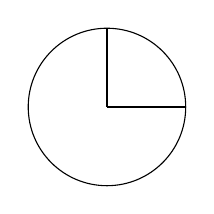
\begin{tikzpicture}
	\draw (0,0) circle (1);
	\draw (0,0) -- (0,1);
	\draw (0,0) -- (1,0);
\end{tikzpicture}

\pause

\begin{lstlisting}
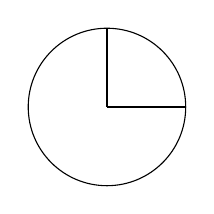
\begin{tikzpicture}
    \draw (0,0) circle (1);
    \draw (0,0) -- (0,1);
    \draw (0,0) -- (1,0);
\end{tikzpicture}
\end{lstlisting}

\end{multicols}
\end{frame}

\subsection{Tracer un arc de cercle}
\begin{frame}[fragile]
\frametitle{Tracer un arc de cercle}
\centering

\begin{tikzpicture}
	\draw (0,0) arc (0:90:1);
\end{tikzpicture}

\begin{lstlisting}
\begin{tikzpicture}
	\draw (0,0) arc (0:90:1);
\end{tikzpicture}
\end{lstlisting}

\end{frame}

\subsection{Ajouter du texte}
\begin{frame}[fragile]
\frametitle{Ajouter du texte}
\centering

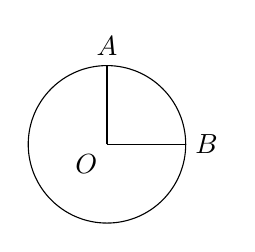
\begin{tikzpicture}
	\draw (0,0) circle (1);
	\draw (0,0) -- (0,1);
	\draw (0,0) -- (1,0);
	\draw (0,0) node[below left]{$O$};
	\draw (0,1) node[above]{$A$};
	\draw (1,0) node[right]{$B$};
\end{tikzpicture}

\pause

\begin{lstlisting}
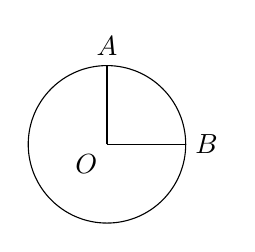
\begin{tikzpicture}
    \draw (0,0) circle (1);
    \draw (0,0) -- (0,1);
    \draw (0,0) -- (1,0);
    \draw (0,0) node[below left]{$O$};
    \draw (0,1) node[above]{$A$};
    \draw (1,0) node[right]{$B$};
\end{tikzpicture}
\end{lstlisting}

\end{frame}

\begin{frame}[fragile]
\frametitle{Ajouter du texte}
\centering

\begin{tikzpicture}
	\draw (1,0) arc (0:135:1);
	\draw (0,0) -- (-1.5,1.5);
	\draw (0,0) -- (2,0);
	\draw (0,0) node[below left]{$O$};
	\draw (70:1) node[above right]{$\frac{3\pi}{4}$};
\end{tikzpicture}

\begin{lstlisting}
\begin{tikzpicture}
    \draw (1,0) arc (0:135:1);
    \draw (0,0) -- (-1.5,1.5);
    \draw (0,0) -- (2,0);
    \draw (0,0) node[below left]{$O$};
    \draw (70:1) node[above right]{$\frac{3\pi}{4}$};
\end{tikzpicture}
\end{lstlisting} 

\end{frame}
 
%----------------------------
%	II - Chemins et options graphiques
%----------------------------

\section{Chemins et options graphiques}
\begin{frame}[fragile]
\frametitle{}

\end{frame}
  
 
%------------------------------------------
%	Questions et Références
%------------------------------------------
 
\begin{frame}
\frametitle{Questions ?}
\begin{center}
\Huge Des questions ?
\end{center}
\end{frame}
 
\begin{frame}
\frametitle{Références}
\begin{itemize}
\item \href{http://paws.wcu.edu/tsfoguel/tikzpgfmanual.pdf }{TikZ and PGF, Manual for version 1.18.\\Par Till Tantau (créateur de TikZ)}
\item \href{http://math.et.info.free.fr/TikZ/bdd/TikZ-Impatient.pdf}{TikZ pour l’impatient.\\Par Gérard Tisseau et Jacques Duma (en français)}
\item \href{http://www.math.uni-leipzig.de/~hellmund/LaTeX/pgf-tut.pdf}{PGF/TikZ - Graphics for LaTeX, A tutorial.\\Par Meik Hellmund (slides)}
\item \href{https://www.coga.tu-berlin.de/fileadmin/i26/download/AG_DiskAlg/FG_KombOptGraphAlg/kappmeier/How_to_TikZ_-_current.pdf}{How to TikZ? An Overview.\\Par Jan-Philipp Kappmeier (slides)}
\end{itemize}
\end{frame}


\end{document}
